\chapter{Methods}\label{chap:methods}

% This creates a chapter and assigns a label so you can reference it elsewhere using \autoref{chap:methods}

This chapter outlines the general procedures used in this study. In a typical dissertation, the Methods chapter should provide enough detail for the study to be replicated, including participants, data acquisition, and analytic procedures.

\section{Study Overview}

% Sections break up your chapter logically

Lorem ipsum dolor sit amet, consectetur adipiscing elit.\supercite{example_reference_1}

% \supercite{} pulls from your .bib file and formats the citation automatically

As illustrated in \textbf{\autoref{fig:example_figure}}, the overall study workflow consists of multiple stages.

% \autoref{} automatically inserts the correct label (e.g., "Figure 1")
% Always reference figures/tables in text before they appear

\begin{figure}[htbp]
    \centering
    % Centers the image

    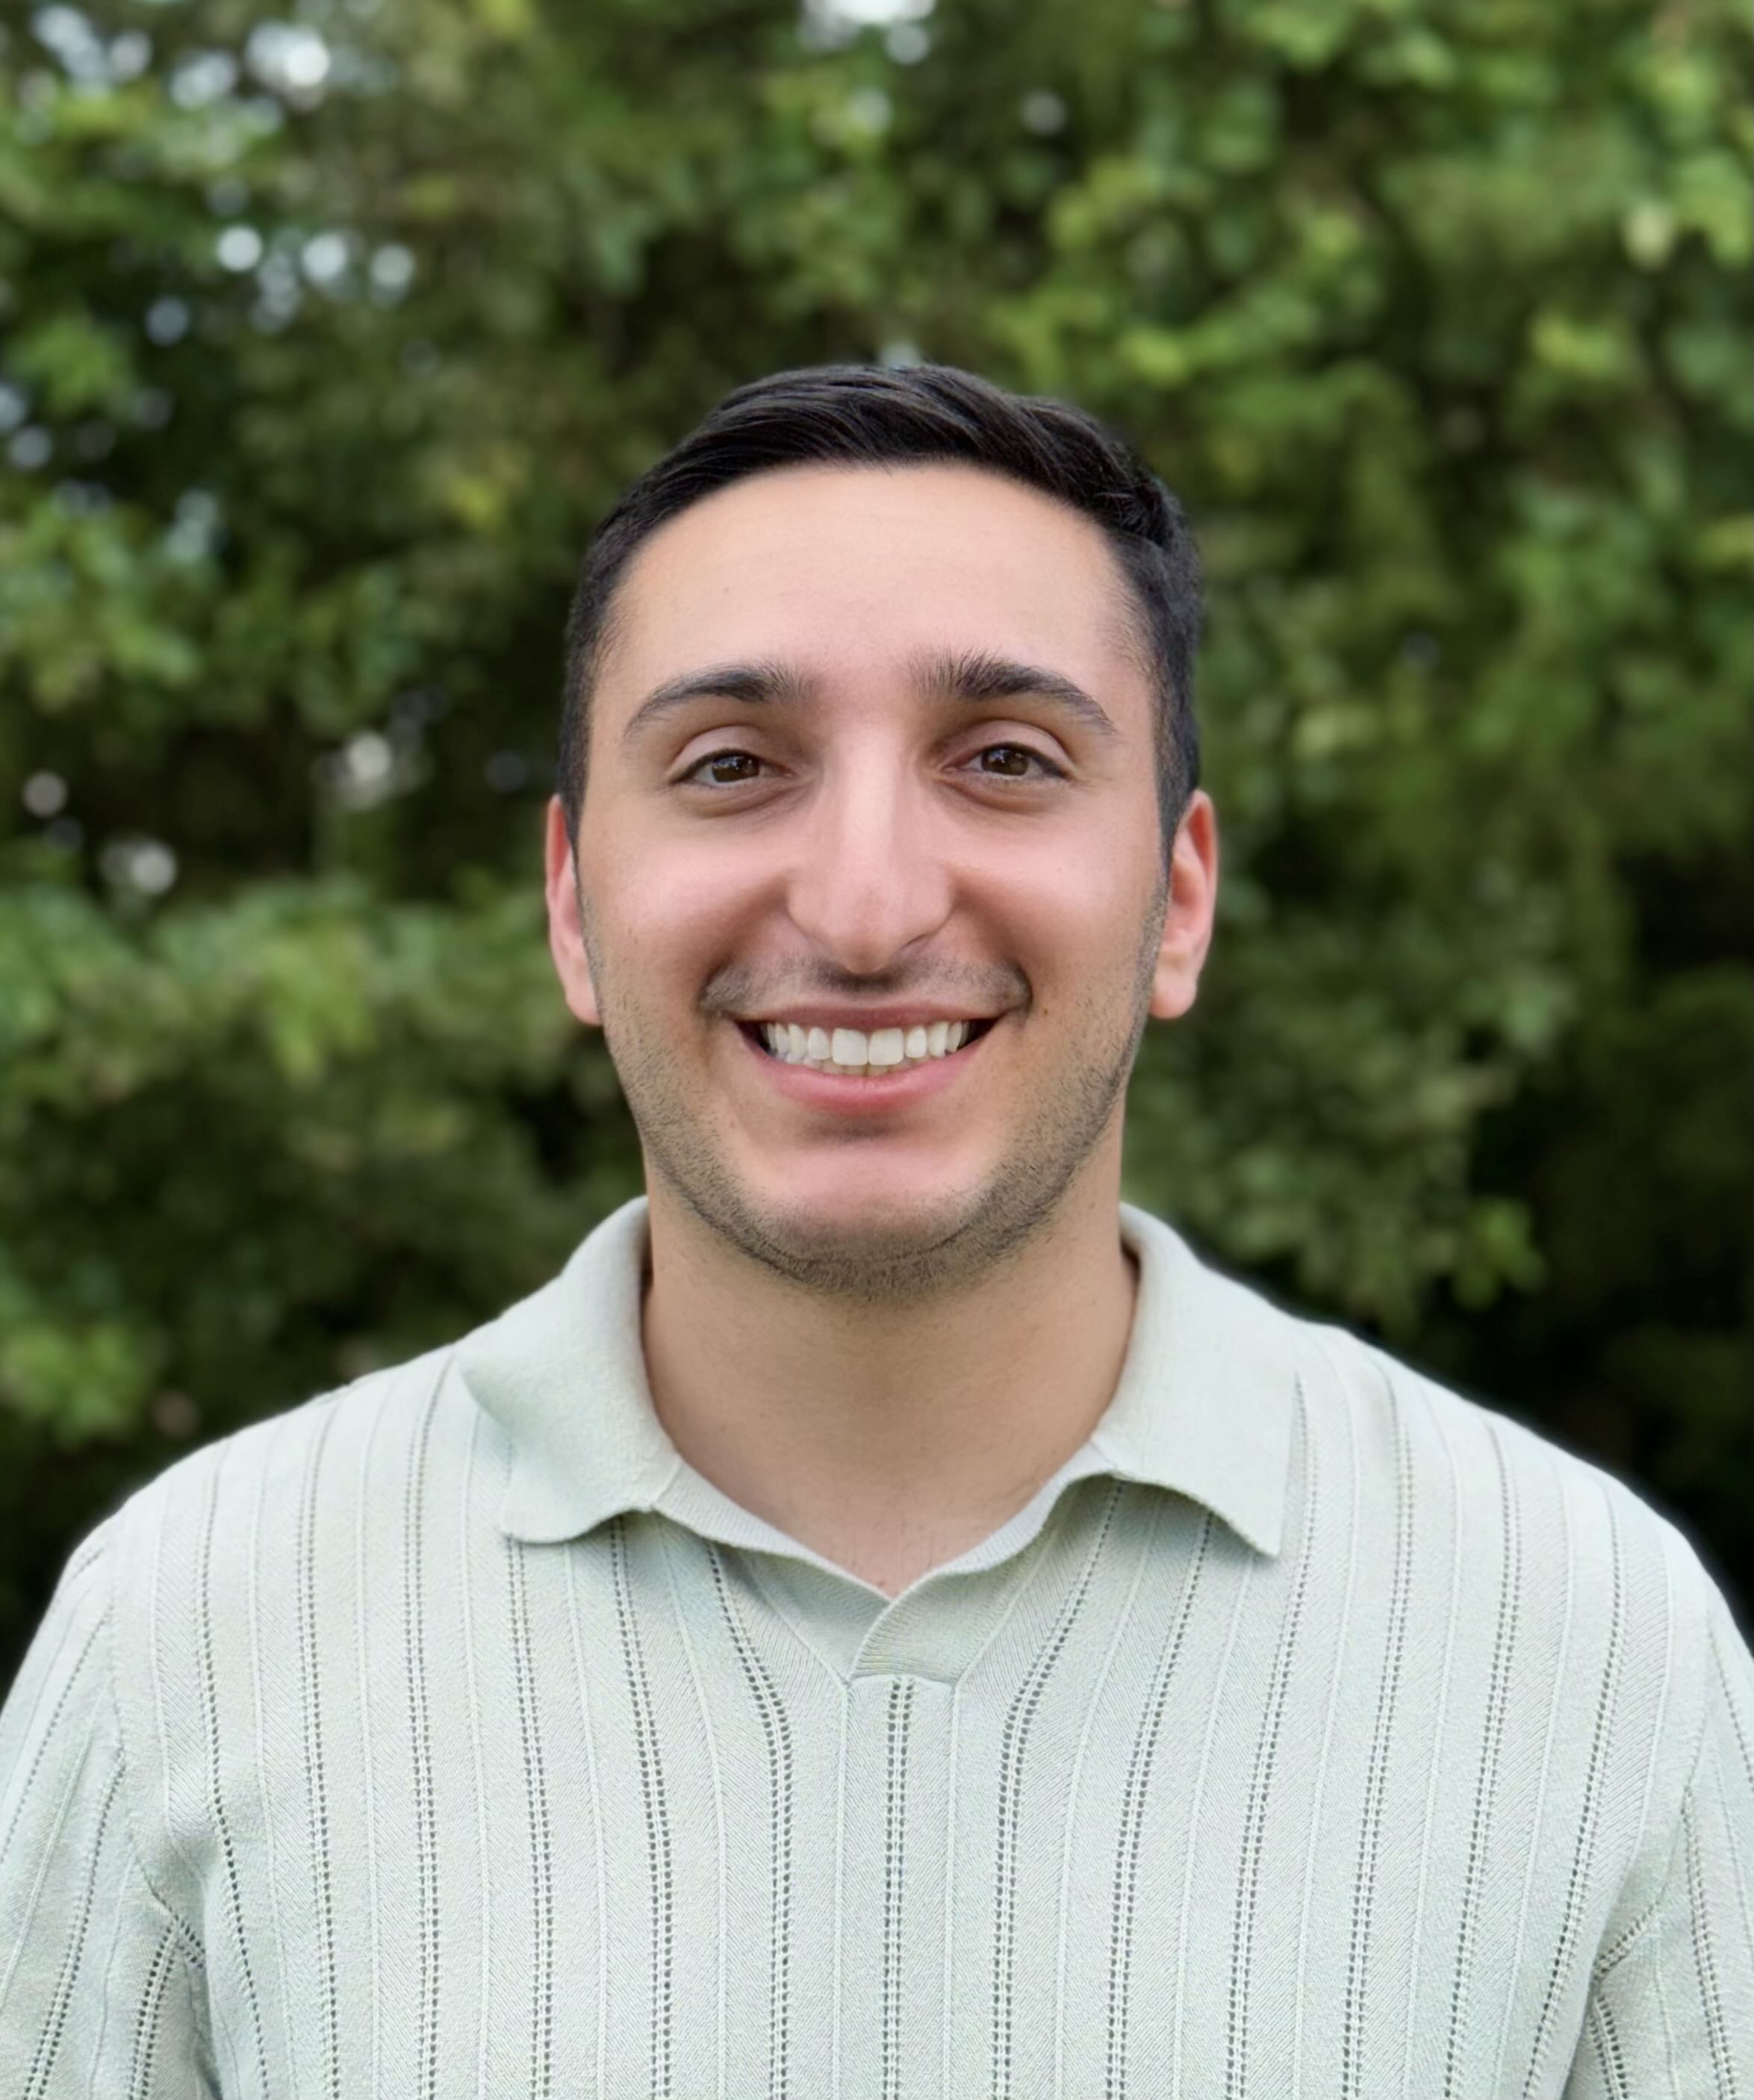
\includegraphics[width=0.5\linewidth]{figures/headshot.png}
    % Includes an image from your figures folder
    % width controls size (0.5 = half the page width)

    \caption[Short caption. This short caption appears in the LIST OF FIGURES]{\textbf{Short caption. This short caption appears in the LIST OF FIGURES} This is the full caption that appears under the figure. Captions should be descriptive enough to understand the figure without referring back to the main text.}
    % Optional [] = short caption for list of figures
    % {} = full caption shown in document

    \label{fig:example_figure}
    % Label MUST come after caption for proper referencing
\end{figure}

\section{Example Section}

Lorem ipsum dolor sit amet, consectetur adipiscing elit.\supercite{example_reference_2}

An example glossary term is \gls{HMSC}.

% \gls{} pulls from your glossary file
% First use = full term, later uses = abbreviated
% In PDFs, this often supports hover/tooltip behavior

Methods chapters often include subsections such as Participants, Data Acquisition, Preprocessing, and Statistical Analysis. These can be created using \texttt{\textbackslash subsection\{\}} to maintain a clear hierarchy.

\subsection{Example Subsection}

Lorem ipsum dolor sit amet, consectetur adipiscing elit.

Example inline math: $p < 0.05$

% Inline math uses $...$ and is embedded within text

Example display math:

\[
y = mx + b
\]

% Display math centers the equation and is used for emphasis or formal definitions

Sed nisi. Nulla quis sem at nibh elementum imperdiet. Duis sagittis ipsum.
